\chapter{Black Holes, White Holes, and Penrose Diagrams}

These notes follow Leonard Susskind's fourth lecture in the supplementary \emph{Topics in String Theory} track of \emph{Cosmology And Black Holes}, with curation by LazyingArt LLC. The lecture begins with a deliberate return to the near-horizon Schwarzschild geometry, then widens the picture: first to an intuitive ``cigar'' interpolation between the horizon and infinity, next to the causal behavior of observers and light rays, then to the singularity and the time-reversed white-hole extension, and finally to Penrose diagrams and the first setup for black-hole formation by collapse.

\section{Near the Horizon: Proper Distance and Hyperbolic Time}

Susskind begins by returning to a construction from the previous lecture. The Schwarzschild radial coordinate \(r\) is replaced by a more physical variable \(\rho\), the proper distance from the horizon, and the Schwarzschild time \(t\) is rescaled to a dimensionless time variable \(\omega\). In the lecture this recap is not ornamental; it is the local datum from which the rest of the global story will grow.

\begin{remark}
Throughout this chapter the lecture's spoken notation \(m,g\) is cleaned to \(M,G\). We also keep a consistent Lorentzian sign convention, even where the spoken transcript briefly stumbles over signs.
\end{remark}

The visible board recap is reproduced below.

\begin{figure}[h]
\centering

\includegraphics[width=0.58\textwidth]{lecture_04_figure_02.png}
\end{figure}

The two explicit equations on the board are
\begin{align}
\omega &= \frac{t}{4MG},\\
ds^2 &= -\rho^2\,d\omega^2 + d\rho^2.
\end{align}
The horizon sits at
\begin{equation}
\rho=0 \qquad \text{when} \qquad r=2MG.
\end{equation}
Susskind does not re-derive the explicit relation \(\rho(r)\) here; he only reminds the audience that \(r\) is \emph{not} the proper distance from the horizon, whereas \(\rho\) is.

The point of the local metric is that it is almost embarrassingly simple. In the two-dimensional radial-time sector, the near-horizon region looks like flat spacetime written in hyperbolic-polar coordinates. To make that statement concrete, Susskind compares it to the Euclidean polar metric
\begin{equation}
ds^2 = \rho^2\,d\theta^2 + d\rho^2,
\end{equation}
and emphasizes that \(\omega\) plays the role of a hyperbolic angle. The only formal difference is the Lorentzian minus sign in front of the angular term.

This is already enough to organize the first causal picture. Lines of constant \(\rho\) are hyperbolae, and the horizon lies at \(\rho=0\). The lecture also distinguishes two notions of horizon that will remain important:
\begin{itemize}
\item the \emph{bifurcate horizon}, namely the special crossing point of the relevant null lines in the local diagram,
\item the \emph{event horizon}, namely the full lightlike boundary beyond which no signal can escape to the exterior.
\end{itemize}

\section{From the Horizon to Infinity: The Cigar Geometry}

The next move is not a new formula but a comparison of regimes. Near the horizon the coefficient of \(d\omega^2\) is \(\rho^2\); very far from the black hole, Susskind wants to know what it becomes. For that he returns to the Schwarzschild metric, suppressing the angular part and keeping only the radial-time sector:
\begin{equation}
ds^2 = -\left(1-\frac{2MG}{r}\right)dt^2 + \frac{dr^2}{1-\frac{2MG}{r}}.
\end{equation}
The spoken lecture briefly fumbles the signs, but the mathematical intent is clear.

\paragraph{Worked asymptotic reduction.}
\begin{enumerate}
\item Take \(r\gg 2MG\).
\item Then \(1-2MG/r \to 1\).
\item Far from the hole, the proper distance from the horizon is approximately the ordinary radius, so \(r\approx \rho\).
\item Hence
\[
ds^2 \approx -dt^2 + dr^2 \approx -dt^2 + d\rho^2.
\]
\item Using \(t=4MG\,\omega\), one obtains
\[
dt^2 = 16M^2G^2\,d\omega^2.
\]
\item Therefore the asymptotic metric becomes
\begin{equation}
ds^2 \approx -16M^2G^2\,d\omega^2 + d\rho^2.
\end{equation}
\end{enumerate}

So the lecture's main geometric comparison is
\begin{align}
ds^2 &\approx -\rho^2\,d\omega^2 + d\rho^2
\qquad \text{near the horizon},\\
ds^2 &\approx -16M^2G^2\,d\omega^2 + d\rho^2
\qquad \text{far away}.
\end{align}
The interesting change is not in the radial piece \(d\rho^2\), but in the time coefficient.

At this point Susskind deliberately leaves spacetime and switches to ordinary space, because the Lorentzian geometry is hard to visualize directly. He asks for an ordinary spatial geometry with metric
\begin{equation}
ds^2 \sim \rho^2\,d\theta^2 + d\rho^2
\qquad \text{near the origin},
\end{equation}
but
\begin{equation}
ds^2 \sim 16M^2G^2\,d\theta^2 + d\rho^2
\qquad \text{far from the origin}.
\end{equation}
His answer is the ``cigar'' geometry: flat near the tip, cylindrical far away. The circumference of the asymptotic cylindrical direction is then
\begin{equation}
\oint ds = \int_0^{2\pi} 4MG\,d\theta = 8\pi MG.
\end{equation}

The lecture's qualitative curvature lesson is attached to this circumference. If \(M\) is large, the asymptotic circle is large, the cigar is blunt, and the tip is less curved. If \(M\) is small, the tip is sharper and the curvature is larger. Susskind does not compute a curvature scalar here; the point is geometric intuition, not a formula beyond the metric itself.

There is also a physical interpretation. The proper-time separation between neighboring values of \(\omega\) depends strongly on position:
\begin{itemize}
\item near the horizon, where \(\rho\) is small, very little proper time elapses for a given \(d\omega\),
\item far away, the same increment of \(\omega\) corresponds to the ordinary asymptotic time interval \(dt=4MG\,d\omega\).
\end{itemize}
This is the lecture's first statement about clocks.

\section{Horizons, Light Rays, and the Outside Observer}

After the cigar analogy, the lecture returns to the Lorentzian causal sketch. The board drawing that supports this part is reproduced below.

\begin{figure}[h]
\centering

\includegraphics[width=0.60\textwidth]{lecture_04_figure_04.png}
\end{figure}

The screenshot preserves the main geometry: two null lines crossing at the bifurcation point, a future wavy singularity curve above, a past wavy singularity curve below, and later-added trajectory lines. Because the handwriting labels are only partly legible, the clean reconstruction below keeps only the secure structure.

\begin{figure}[h]
\centering
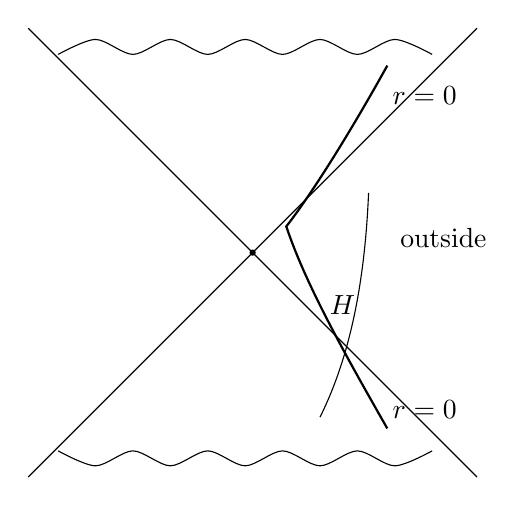
\begin{tikzpicture}[scale=0.95]
\draw (-3,-3) -- (3,3);
\draw (-3,3) -- (3,-3);

\draw plot[smooth] coordinates {(-2.6,2.65) (-2.1,2.85) (-1.6,2.65) (-1.1,2.85) (-0.6,2.65) (-0.1,2.85) (0.4,2.65) (0.9,2.85) (1.4,2.65) (1.9,2.85) (2.4,2.65)};
\draw plot[smooth] coordinates {(-2.6,-2.65) (-2.1,-2.85) (-1.6,-2.65) (-1.1,-2.85) (-0.6,-2.65) (-0.1,-2.85) (0.4,-2.65) (0.9,-2.85) (1.4,-2.65) (1.9,-2.85) (2.4,-2.65)};

\fill (0,0) circle (1.2pt);

\draw[thick] (1.8,2.5) .. controls (1.3,1.6) and (0.8,0.8) .. (0.45,0.35)
             .. controls (0.7,-0.4) and (1.2,-1.3) .. (1.8,-2.35);

\draw (0.9,-2.2) .. controls (1.3,-1.4) and (1.5,-0.4) .. (1.55,0.8);

\node at (1.2,-0.7) {$H$};
\node at (2.3,2.1) {$r=0$};
\node at (2.3,-2.1) {$r=0$};
\node at (2.55,0.2) {outside};
\end{tikzpicture}
\end{figure}

The key reading rule is simple and is repeated throughout the lecture:

\begin{definition}
In the causal sketches used here, radial light rays are drawn at \(45^\circ\).
\end{definition}

That rule makes the meaning of the event horizon immediate. An inward null ray can cross the horizon into the black-hole interior, but an outward null ray emitted from the interior never reaches the outside world. This is the operational definition Susskind wants the audience to carry: the event horizon is a one-way signaling barrier.

The other central ingredient is the family of fixed-\(\rho\) outside worldlines. These represent observers who hover at a fixed proper distance from the horizon. For such an observer, Schwarzschild time and the lecture's dimensionless time are related by
\begin{equation}
t = 4MG\,\omega.
\end{equation}
Susskind then personifies one such observer as Bob, stationary outside the black hole, and uses him to organize the rest of the causal story.

\section{Bob, Alice, Redshift, and the One-Way Barrier}

Once Bob is in place, the lecture becomes explicitly operational. Alice falls toward the horizon while Bob remains outside. The question is not merely what Alice \emph{does}, but what Bob \emph{sees}.

Because Bob receives signals only along his past light cone, he sees Alice at progressively earlier points of her worldline. As he continues to wait outside, he sees fewer and fewer of her waves per unit of his own proper time. In the idealized classical picture she appears to freeze just outside the horizon; more precisely, he never sees her cross it.

The lecture then sharpens the visual statement into a frequency statement. Alice is seen only through the light emitted by the motion of her charges, so Bob sees those oscillations slow down. Optical light becomes infrared, infrared becomes long-wavelength radio, and in practice Alice fades from view. This is the physical content of the large redshift at the horizon.

Alice's point of view is very different. She continues to see Bob even after she herself has crossed the horizon. Bob can still send signals inward to her, but she can no longer send signals outward to him. The asymmetry is the point: Bob sees Alice redshift and disappear, while Alice sees Bob receding and redshifting, but not vanishing at horizon crossing.

The lecture then uses a particularly memorable refinement: Alice falls feet first. Her feet cross the horizon before her head. If she simply continues to fall, nothing locally singular happens at the horizon. She continues to receive light from her feet, just as she receives light from any nearby part of her body: always from slightly earlier points on their worldlines.

But if she decides to keep her head outside after her feet have crossed the horizon, the story changes. To stay out, her head must accelerate away from the black hole. In the lecture's description, the part already behind the horizon cannot accelerate enough to keep up. What was a finite body becomes stretched farther and farther in the accelerated frame, until the body is torn apart. In this argument the horizon is not a place of local catastrophe for free fall; it is a place that makes hovering impossible once part of the system has already crossed.

\section{The Singularity, Coordinate Interchange, and the White Hole}

Only after the horizon story is established does Susskind turn to the singularity. He rewrites the radial-time Schwarzschild metric and asks what changes at \(r=2MG\). The answer is not that the horizon is singular, but that the coordinate roles of \(t\) and \(r\) interchange there.

The clean statement is:
\begin{equation}
1-\frac{2MG}{r}>0 \quad \text{for } r>2MG,
\qquad
1-\frac{2MG}{r}<0 \quad \text{for } r<2MG.
\end{equation}
Thus outside the horizon the \(dt^2\) term is timelike and the \(dr^2\) term spacelike, while inside they exchange their signs. Susskind is careful here: this does \emph{not} mean that something physically dramatic happens at the horizon itself. It is a peculiarity of Schwarzschild coordinates, not a curvature singularity.

The truly dramatic place is
\begin{equation}
r=0.
\end{equation}
That is the singularity. In the lecture's diagram it appears not as an ordinary location one might orbit around, but as a future boundary, drawn as a hyperbola-like spacelike curve. Once a timelike or null worldline has crossed the future horizon, its future lies toward that singular boundary. The point is not merely that no signal escapes; the point is that no future-directed escape route exists at all.

Susskind then extracts a second consequence from the same metric. Since Schwarzschild is time-independent, it is invariant under the reversal \(t\to -t\). Running a consistent infall history backward therefore produces another mathematically allowed history. In the reversed history, matter does not fall through a future horizon into a future singularity; instead it emerges from a past singularity through a past horizon. This time-reversed object is the \emph{white hole}.

The lecture treats this extension as mathematically present but physically suspect. One can pass into the future horizon just as one can emerge from the past horizon in the time-reversed picture, but the reversed process looks absurd from the outside: Bob sees an object suddenly ejected from a singular past. The equations allow it, but the physical world does not present it to us as an ordinary occurrence.

\section{Entropy and Why the White Hole Is Not a Real Astrophysical Object}

At this stage Susskind does not deny the white hole mathematically; instead he denies it statistically. General relativity is time-reversal invariant, so one cannot rule out the white-hole half of the eternal Schwarzschild diagram by equations alone. One must appeal to the same logic that distinguishes ordinary irreversible phenomena from their fantastically tuned time reverses.

This is why the lecture turns to examples: the bomb that explodes rather than reassembles itself, the ball that rolls down the hill rather than balancing itself at the top, the billiard balls that scatter rather than spontaneously reforming a perfect triangle, and the ice cube that melts in hot water rather than assembling itself out of thermal agitation. All of these reversed histories are dynamically possible in principle, but they are entropically implausible.

The same argument is then transferred to black holes. The horizon has entropy. It encodes hidden microscopic information. A white hole would amount to the black-hole horizon or singular past organizing itself into an extraordinarily special low-entropy outward burst---for instance, the sudden ejection of a complete Alice. The lecture's verdict is not that this is forbidden by a theorem stronger than the equations; the verdict is that it is an extreme fluctuation, on the same conceptual footing as an ice cube spontaneously emerging from a hot pot.

So the white-hole half of the eternal Schwarzschild solution is retained as a mathematical extension, but it is downgraded as a model of actual astrophysical black holes.

\section{Penrose Diagrams and the Global Picture}

After the break Susskind pauses to clarify the jargon of \emph{proper distance}. The secure content of that clarification is simple: proper distance is the distance measured by actual meter sticks along the chosen spatial path. That reminder matters because the next construction is global rather than local.

\begin{definition}
A Penrose diagram is a compactified spacetime diagram in which an infinite spacetime region is mapped to a finite domain, while radial null rays remain at \(45^\circ\).
\end{definition}

Susskind begins with flat spacetime, not with the black hole. He takes the half-plane with coordinates \((t,\rho)\), where \(\rho\ge 0\), and draws a grid of constant \(t\) and constant \(\rho\). The construction-stage board evidence is reproduced below.

\begin{figure}[h]
\centering

\includegraphics[width=0.58\textwidth]{lecture_04_figure_05.png}
\end{figure}

The more complete board diagram from the same discussion is:

\begin{figure}[h]
\centering

\includegraphics[width=0.62\textwidth]{lecture_04_figure_06.png}
\end{figure}

The lecture's point is that the whole infinite half-plane can be squashed into a finite triangular region. A clean schematic version is shown next.

\begin{figure}[h]
\centering
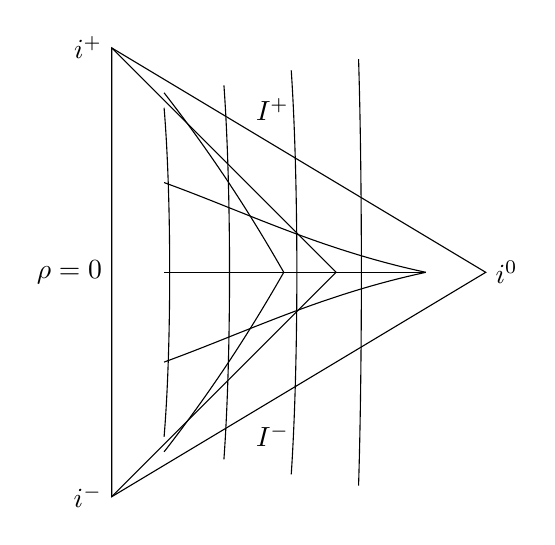
\begin{tikzpicture}[scale=0.95]
\draw (0,-3) -- (0,3) -- (5,0) -- cycle;

\draw (0.7,-2.4) .. controls (1.4,-1.5) and (1.9,-0.7) .. (2.3,0);
\draw (0.7,2.4) .. controls (1.4,1.5) and (1.9,0.7) .. (2.3,0);

\draw (0.7,-1.2) .. controls (1.8,-0.8) and (2.8,-0.3) .. (4.2,0);
\draw (0.7,0) .. controls (1.8,0.0) and (2.8,0.0) .. (4.2,0);
\draw (0.7,1.2) .. controls (1.8,0.8) and (2.8,0.3) .. (4.2,0);

\draw (0.7,-2.2) .. controls (0.8,-1.0) and (0.8,1.0) .. (0.7,2.2);
\draw (1.5,-2.5) .. controls (1.6,-1.1) and (1.6,1.1) .. (1.5,2.5);
\draw (2.4,-2.7) .. controls (2.5,-1.2) and (2.5,1.2) .. (2.4,2.7);
\draw (3.3,-2.85) .. controls (3.35,-1.25) and (3.35,1.25) .. (3.3,2.85);

\draw (0,-3) -- (3,-0);
\draw (0,3) -- (3,0);

\node[left] at (0,3) {$i^+$};
\node[left] at (0,-3) {$i^-$};
\node[right] at (5,0) {$i^0$};
\node[above right] at (1.8,1.9) {$\mathscr{I}^+$};
\node[below right] at (1.8,-1.9) {$\mathscr{I}^-$};
\node[left] at (0,0) {$\rho=0$};
\end{tikzpicture}
\end{figure}

Here the left boundary is the timelike axis \(\rho=0\), the right tip is spatial infinity \(i^0\), the upper and lower slanted edges are future and past null infinity \(\mathscr{I}^\pm\), and the upper and lower endpoints of the left boundary are timelike future and past infinity \(i^\pm\).

Once the audience has learned to read the flat-space Penrose diagram, the black-hole diagram can be compactified in the same spirit. The eternal Schwarzschild geometry contains:
\begin{itemize}
\item an exterior region,
\item a future singularity,
\item a past singularity,
\item a second asymptotic exterior region,
\item horizons separating these regions.
\end{itemize}
A clean schematic version, matching the lecture's discussion rather than claiming a board-perfect transcription, is:

\begin{figure}[h]
\centering
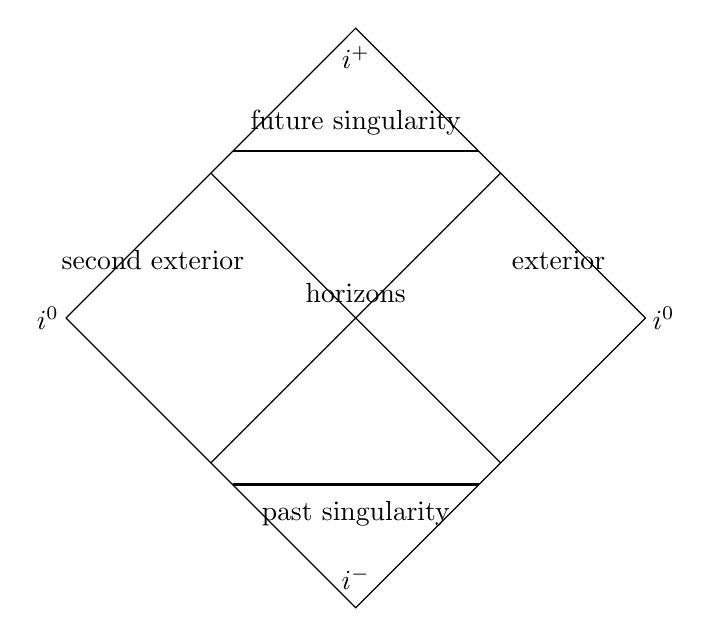
\begin{tikzpicture}[scale=0.92]
\coordinate (L) at (-4,0);
\coordinate (R) at (4,0);
\coordinate (TL) at (-2,2);
\coordinate (TR) at (2,2);
\coordinate (BL) at (-2,-2);
\coordinate (BR) at (2,-2);
\coordinate (C) at (0,0);

\draw (L) -- (TL) -- (0,4) -- (TR) -- (R);
\draw (L) -- (BL) -- (0,-4) -- (BR) -- (R);

\draw (TL) -- (C) -- (TR);
\draw (BL) -- (C) -- (BR);

\draw[thick] (-1.7,2.3) -- (1.7,2.3);
\draw[thick] (-1.7,-2.3) -- (1.7,-2.3);

\node at (0,2.7) {future singularity};
\node at (0,-2.7) {past singularity};
\node at (2.8,0.8) {exterior};
\node at (-2.8,0.8) {second exterior};
\node at (0,0.35) {horizons};
\node at (0,3.6) {$i^+$};
\node at (0,-3.6) {$i^-$};
\node at (4.25,0) {$i^0$};
\node at (-4.25,0) {$i^0$};
\end{tikzpicture}
\end{figure}

The lecture's interpretive payoff is immediate. A radial light ray entering the black-hole region terminates on the future singularity. The second exterior region is mathematically present, but no causal signal connects it to the exterior region in which Bob lives. This is why Susskind calls the fully eternal picture physically misleading: it is the geometry of a black hole that was somehow always there.

\section{Real Black Holes, Newton's Theorem, and Birkhoff's Theorem}

The lecture closes by pivoting away from eternal black holes. Real black holes are formed. One can imagine diffuse matter, even a cloud of photons, entering from far away. Enough energy concentrated in a sufficiently small region will gravitate strongly enough to make a black hole. The question is how to splice the pre-collapse geometry to the post-collapse geometry.

To prepare that construction, Susskind introduces Newton's shell theorem in a deliberately operational language of lines of force. The theorem says that for a spherically symmetric shell of mass:
\begin{itemize}
\item the field inside the shell vanishes,
\item the field outside the shell is exactly the same as the field of a point mass at the center.
\end{itemize}
He also emphasizes that the same conclusion remains true if the shell changes size in time, provided the total mass is conserved.

The general-relativistic version is Birkhoff's theorem in the simple form needed for the next lecture.

\begin{theorem}[Birkhoff's theorem in the form used in the lecture]
For a spherically symmetric shell of total mass \(M\), the spacetime inside the shell is flat Minkowski space, while the spacetime outside the shell is the Schwarzschild geometry of mass \(M\).
\end{theorem}

Thus the two pieces to be patched together are
\begin{align}
ds^2_{\text{inside}} &= -dt^2 + dx^2 + dy^2 + dz^2,\\
ds^2_{\text{outside}} &= \text{Schwarzschild}(M).
\end{align}
As the shell collapses, the total mass does not change; only the radius of the shell changes. The lecture stops here on purpose. The theorem has been stated, the two geometries are known, and the next task will be to join them into a simple model of black-hole formation.

\section{Summary}

The lecture begins locally and ends globally. Near the horizon, the Schwarzschild geometry is flat spacetime in hyperbolic-polar disguise, with \(\rho\) measuring proper distance from the horizon and \(\omega=t/(4MG)\) the corresponding dimensionless time. Moving outward changes the coefficient of the time term, and Susskind uses the cigar analogy to make that variation geometrically visible.

From there the lecture turns causal: horizons are one-way barriers, Bob and Alice do not describe the same visual story, and once the singularity is included, horizon crossing becomes not only a loss of communication but a loss of any future escape route. The time-reversed white-hole half is mathematically present but entropically implausible. After the break, Penrose diagrams compress the infinite spacetime into readable finite pictures, and the lecture ends by setting up the next problem: replace the eternal black hole by a collapsing shell, with flat spacetime inside and Schwarzschild outside.